\section{Database}
\label{sec:database}

Now we can specify the foundational data collection structure we will use, which is a database. And beyond that, the relation of the database with the knowledge manager and why we should use it.

% --------------------------------------------------
\subsection{Database}
\label{ssec:database}

\ac{DB}\index{database} is the most used way or structured set to organize collection of information that can be accessed, managed, updated, deleted, and others.
It is also can be programmed as such.
We involve database system and \ac{DBMS} to take care of our database.
Note that even database is principally organize information, we can utilize it to organize knowledge if the upper layer we configure database as the storage while interacting with the database is designed for managing traffic of knowledge.

% --------------------------------------------------
\subsection{Database System}
\label{ssec:database-system}

\ac{DBS}\index{database system} is a computerized record keeping system with the overall purpose of maintaining information and making it available whenever required.
The \ac{DBS} typically stores related data in a computer system.~\autocite{Foster2014Intro}

% --------------------------------------------------
\subsection{Database Management System}
\label{ssec:dbms}

\ac{DBMS}\index{database management system|see{DBMS}} is a set of programs that allow for the
management of a database.~\autocite{Foster2014Intro}
In short, it is the database program, the software system that uses a standard method of cataloging, retrieving, and running queries on data. \ac{DBMS} manages incoming data, organizes it, and provides ways for the data to be modified or extracted by users or other programs.~\autocite{TechTerms:2014:DBMS}
Most popular \ac{DBMS} used today are categorized in an \ac{SQL} database and \ac{NoSQL} database.

% --------------------------------------------------
\subsection{NoSQL Database}
\label{ssec:nosql-db}

\ac{NoSQL}\index{not only SQL|see{NoSQL}} database, the counterpart of \ac{SQL}\index{Structured Query Language|see{SQL}} database, is a a set of concepts that allows the rapid and efficient processing of data sets with a focus on performance, reliability, and agility.~\autocite{McCreary2014NoSQL}
It embraces the broad variety of different cases that require more ways to manage database specially in the differentiation of data volume, objective view and close similarity with real world, the access frequency, and demand of higher perfornace.

\ac{NoSQL}\index{NoSQL} model can be much better or suitable than SQL\index{SQL} in terms of managing data that is cannot be modeled after table or there is no need for relation between each data.
Moreover, \ac{NoSQL} often not using a schema or entity-relational model as its primary data model, so the data model is flexible enough to be modified with ease later.
Even though, it is still important to pay attention to schema that is formed by creating the data inside \ac{NoSQL} database.
This way of storing data can storae and retrieve data that is other than in tabular form and without relation.
There are various types of NoSQL databases for and some examples of them:

\begin{easylist}
  & Document databases: MongoDB, CouchDB, RethinkDB
  & Graph databases: Neo4J, FlockDB, GraphBase
  & Key-value/tuple databases: Redis, Riak, RocksDB
  & Wide column databases: Cassandra, Hadoop, Informix
  & Multimodel databases: ArangoDB, OrientDB, Datomic, FoundationDB
  & Object databases: Versant, VelocityDB, ObjectDB
  & XML databases: BaseX, eXist, Sedna
  & Multidimensional databases: SciDB, MiniM DB, rasdaman
  & Multivalue databases: U2, OpenQM, Tieto TRIP
  & and others such as event sourcing and network model
\end{easylist}

% --------------------------------------------------
\subsection{Document Database}
\label{ssec:document-database}

With many \ac{NoSQL} database types available, one of them and most popular is document database\index{document database}, a database that oriented for processing pair of  key with a complex data structure known as a document.
Documents can contain many different key-value pairs, or key-array pairs, or even nested documents.~\autocite{MongoDB:2015:NoSQL}
Document database itself by design is really resemble the real-world data as we seen daily, it is the best fit if we need to store complex information with key and value model.
Especially needed when there should be a high linear scalability and schema flexibility of the data model.
For example, we can see that a voucher, ticket, letter, invoice, are all documents consist of label and field which equate with key and complex data value.

\begin{figure}[htbp]
    \centering
    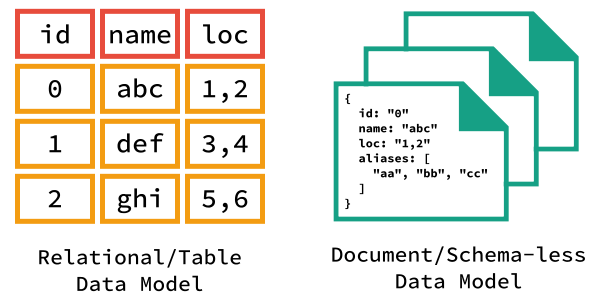
\includegraphics[width=8cm]{\dir/include/data-model.png}
    \caption[Relational vs Document Data Model]{Compared illustration of relational vs document data model}
    \label{fig:data-model}
\end{figure}

As shown in \autoref{fig:data-model}, relational data model use table approach to store the data.
While document data model is mostly represented as a documents to store collection of complex documents with various, could be arbitrary, and nested formats.

% --------------------------------------------------
\subsection{Reason of Using Database}
\label{ssec:reason-db}

As we know prior of computer system, knowledge management has been around for a long time.
But the manual process of managing and transferring knowledge in such a traditional way like writing down on paper or board, speaking in person, communicating via phone or chat are not effective and efficient.
Therefore although those ways of doing can also be continued or complemented, requisite of doing it faster and easier is recommended to use completely the help of a database-powered \ac{KMS}.
